\section{Methodology}

\subsection{Dataset, Missing-ness Analysis and Imputation}
\subsubsection{Data Alignment, Harmonization and Quality Check}
The foundation of this study is a composite dataset created by merging two extensive open-source thermal comfort repositories: the ASHRAE Global Thermal Comfort Database II (ASHRAE II) \cite{foldvary2018ashrae} and the Chinese Thermal Comfort Datasets (Chinese DB) \cite{yang2023chinese}. These datasets span different historical periods, with ASHRAE II containing records from 1983 to 2022 and the Chinese DB covering 2010 to 2023. Recognizing significant overlap in contributors and research aims, we undertook a harmonization process. We successfully reconciled 29 core variables where definitions largely overlapped (see Appendix~\ref{sec:alignment} for list), although challenges remained due to differing categorical definitions (e.g., \texttt{coolingsys}, \texttt{building\_type}) between the sources. Specific harmonization steps included mapping geographic and climatic information (\texttt{city}, \texttt{country}, \texttt{climate\_zone}) from ASHRAE II's accompanying metadata and leveraging the \texttt{geopy} library \cite{Geopy} to derive latitude and longitude for entries in the Chinese DB. A detailed column harmonization mapping table is, once again provided in \ref{sec:alignment}. This process yielded a combined dataset exceeding 150,000 records.

Initial analysis revealed substantial missing data, with Figure~\ref{fig:completeness} illustrating the fill ratio per variable. While essential environmental variables like air temperature ($t_a$) showed high completeness, crucial inputs for standard models (e.g., PMV) exhibited significant missingness (approx. 10.6\% across the six core PMV inputs), and the overall missingness across the harmonized dataset reached approximately 33\%. Personal contextual factors (\texttt{age}, \texttt{gender}, \texttt{height}, \texttt{weight}) displayed even higher missingness rates, ranging from 30\% to 70\%. Figure~\ref{fig:hexmap} further highlights that data completeness has improved over time but remains a persistent issue even in recent records.

\begin{figure}[h!]
    \centering
    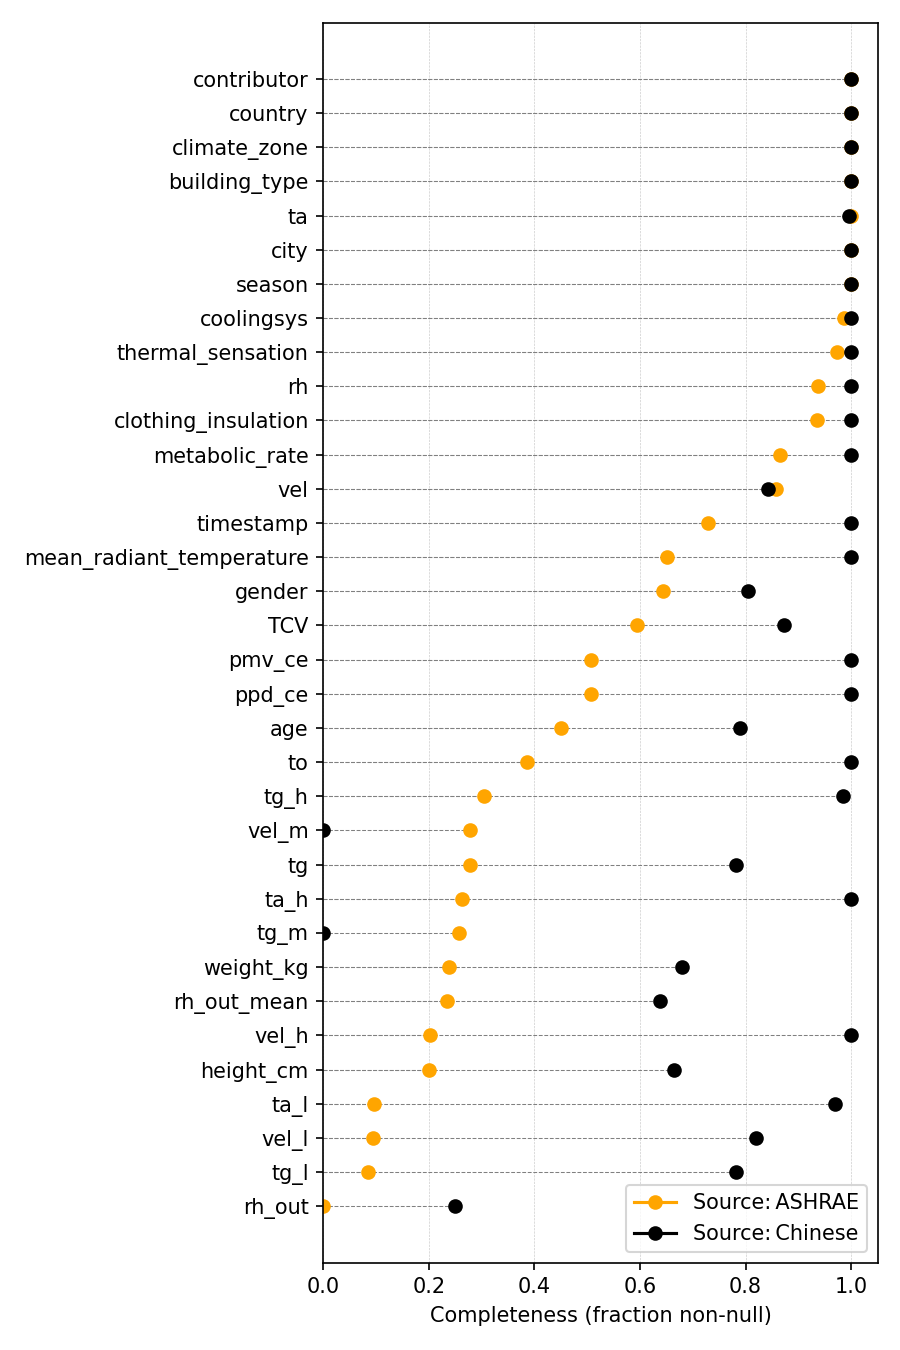
\includegraphics[width=0.5\linewidth]{fig/completeness.png}
    \caption{Fill ratio by column present in the columns we filled}
    \label{fig:completeness}
\end{figure}

Examining Figure~\ref{fig:completeness} further, we noticed that even for the 6 columns that are required to calculate PMV values, there are a total of 10.6\% of fields that are missing. Expanding this to the harmonized combined dataset altogether, this percentage raises up to 30\%. For fields that are more associated personal contextual factors, such as \texttt{age, gender, height, weight}, their respective `missing' percentage ranges from 30\% to up to 70\% in certain cases. 

\begin{figure}[h!]
    \centering
    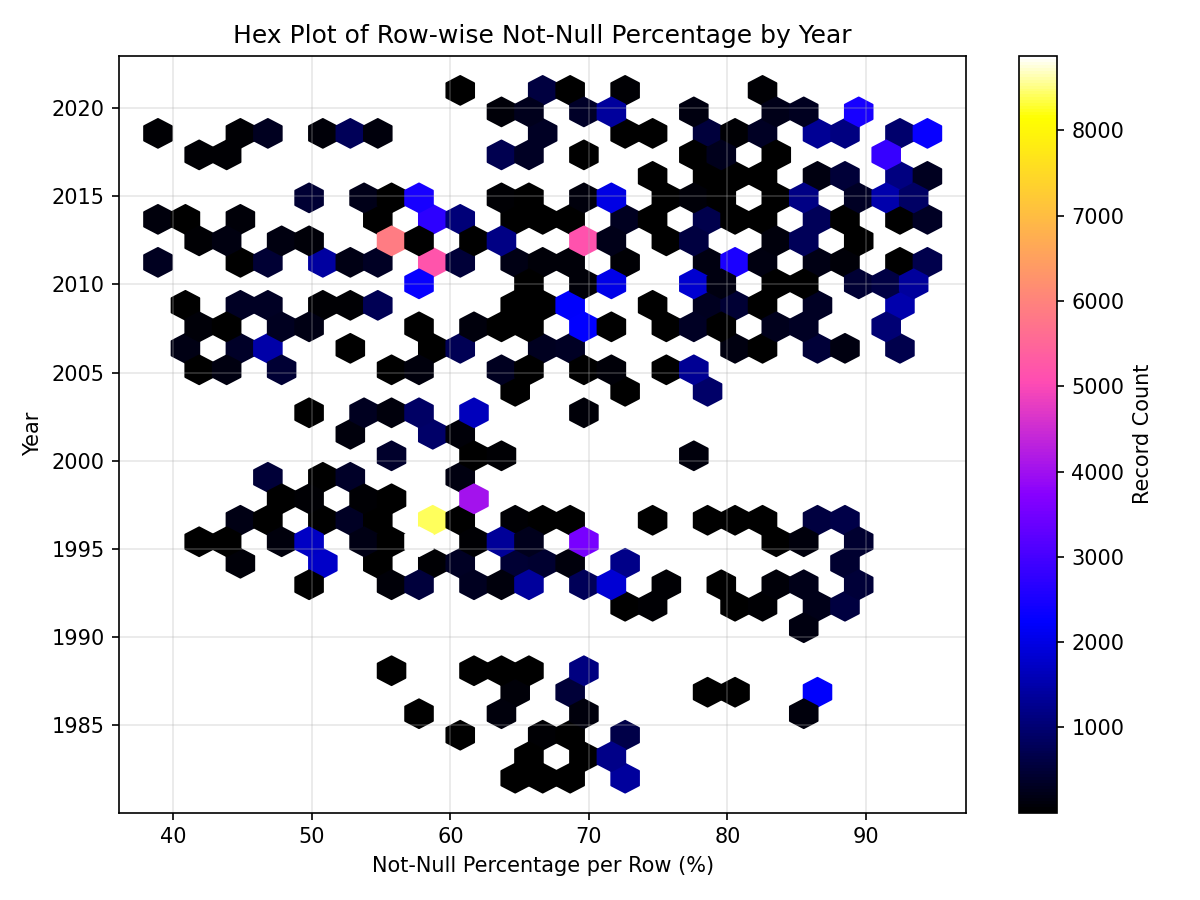
\includegraphics[width=0.75\linewidth]{fig/hex_fill.png}
    \caption{Percentage of columns filled hexagonal bin plot across all yaers data was available}
    \label{fig:hexmap}
\end{figure}

Attempting to enhance the predictive power of the combined dataset, we also leveraged \texttt{geopy} package to construct additional features such as latitude and longitude from the city names in the Chinese DB which were not initially available. Similarly, we mapped back the city, country and climate zone from ASHRAE's accompanying metadata to better align the two dataset, hence the much higher `fill-ratio' of these values in Figure~\ref{fig:completeness}. Not only are more granular measurement details such as velocities, air temperature and globe temperature at different heights (`\_l', `\_m', `\_h', etc. ), necessary inputs that are crucial to predicting condition-specific PMV values are not always available. 

\subsubsection{Missing Completely At Random (MCAR) Validity Analysis}\label{sec:MAR_Validation}
We visualized the missing data pattern over the years for across all variables in Figure~\ref{fig:completeness}. We tested the hypothesis that missingness to see whether they are  dependent on other observed variables, which would provide evidence against the Missing Completely At Random (MCAR) assumption with chi-squared, t-tests and multivariate logistic regression of the field-specific missingness. 

There is one crucial step that we needed to complete before attempting to suggest to assemble the method surrounding our proposed projected values of the missing data: identify the missingness mechanism to make sure the imputation is something an architecture like VAE could tackle. To do this, we validated the missing data mechanism. Following Rubin's classification \cite{Rubin1976}, we tested the hypothesis that the data were Missing Completely At Random (MCAR). Univariate associations between missingness indicators and observed predictors were evaluated using Chi-squared tests (for categorical predictors) and independent samples t-tests (for numerical predictors). Additionally, multivariate logistic regression models were built to predict missingness using all relevant observed variables, with model performance assessed via the Area Under the Receiver Operating Characteristic Curve (ROC AUC) and reported to assess the MCAR validity.

% There is one crucial step that we needed to complete before attempting to suggest to assemble the architecture surrounding our proposed filing of the missing data: identify the missingness mechanism to make sure the imputation is something an architecture like VAE could tackle. According to Rubin's definition of missing data mechanism aka response mechanism, every data point has some likelihood of being missing, and the processes that governs these probabilities can generally be categories as missing completely at random, missing at random, and missing not at random. %Explain this theory better...?
% Validating the missingness of the data has randomness that can be imputed through the variational inference and probablistic learning that a model like VAE promises is a crucial `go-nogo' goal post for our investigation to continue. To assess the randomess of the data at hand, we conducted a MAR validity check to assess whether data fields missing is indeed completely random.  
\subsubsection{Missing Data Imputation Using VAE}
With MCAR validity established (Section~\ref{sec:MAR_Validation}), we then employed a VAE integrated within a Physics-Informed Neural Network framework (PINN-VAE, see Section~\ref{sec:PINN_VAE_Arch}) for simultaneous imputation of projected values. The VAE component learns a probabilistic latent representation of the data, enabling the reconstruction of missing values based on observed patterns and has been shown to effectively impute missing data under \gls{mcar} validity\cite{vanbuuren2018flexible}.

The PINN-VAE model was trained using the Adam optimizer \cite{Kingma2014Adam} with a learning rate of $1 \times 10^{-4}$ for 50 epochs and a batch size of 64. L2 gradient clipping at a threshold of 1.0 was applied for stability. The latent space dimensionality was set to 8, selected based on preliminary experiments evaluating validation loss across dimensions \{4, 8, 16\}. The KL divergence term in the VAE loss function (Eq.~\ref{eq:kloss}) was assigned a weight of 0.1. The physiology-related loss components (Eq.~\ref{eq:phys_loss}) collectively received a weight of $\lambda_{phys}=0.33$, ensuring physiologically plausible imputations and intermediate predictions (detailed in Section~\ref{sec:Physiological_Constraints}).

A separate validation strategy focused solely on imputation accuracy (e.g., using artificially masked data) was not performed. The primary benchmark, LightGBM \cite{ke2017lightgbm}, inherently handles missing values and demonstrates strong performance by potentially learning from missingness patterns. Our approach compares the explicit, constrained imputation of PINN-VAE directly against this implicit handling baseline, rather than optimizing imputation accuracy in isolation. Assessing imputation performance on artificially masked data was thus considered less relevant for the core comparison and goals of this study.

\subsection{PINN-VAE Architecture}\label{sec:PINN_VAE_Arch}
Physics-Informed Neural Network is a concept that is still somewhat new to a lot of researchers coming from traditional engineering educational background. Where PINN originated from, the neural networks on the other hand, are known to demonstrate strength with larger datasets, especially with data of great quality and have been applied in many studies on the built environment leveraging techniques like \gls{cnn}, \gls{gnn}, etc. Variationa AutoEncoders, on the other hand has shown great premises of application in distribution-following data imputation. While both VAEs and PINNs have been independently applied in other domains, their combination is especially suited here: the VAE handles missing tabular inputs by learning a latent representation of the dataset, while the PINN structure constrains intermediate outputs to remain biophysically plausible. This synergy allows our model to simultaneously impute, predict, and regulate according to known physiology. %Source and cite this

However, since neural network models (NNs from hereon) are known to lack clear explainability or interpretability of inferencing, leading to a lack of trust in how it handle explicit tasks where critical decisions need to be made upon, limiting their usages solely to design and optimization of systems rather than becoming an actual feedback loop control signal. 
The emergence of PINN alters that image of NNs as it ties the black models directly to physical constraints and governing equations, putting constraints on how the model should learn from the training data provided. 

As a rising field of interests, PINN are now seeing a much wider usage in the engineering domain and generating more trust amongst researchers who faces challenges that they need to address in the real world instead. To fully embrace the power of PINN models, however, the dataset needs to have no null values just like most of the other NNs, hence with the current combined datset, PINN alone will not suffice: we need another piece to complete the puzzle.

VAE, or Variational Auto-encoder, is the piece we identified that would-rise up to the challenge. As the name suggests, VAE incorporates the benefit of both an autoencoder architecture and the assumption of an underlying probabilistic latent distribution. This learning process, termed as Variational Inference (VI) enables the NN to learn meaning compressed representations, i.e. latent variables \gls{zlatent} of complex data\cite{Kingma2013VAE,Kingma2019IntroVAE}, as we're demonstrating in Figure~\ref{fig:diagram-losses}. 


Putting it into the perspective through the corresponding netowrk is showing, the VI process learns the underlying distribution in $\epsilon \sim \mathcal{N}(0, 1)$. To put it into a clearer perspective, he raw feature vector $\mathbf{x}$ (environmental, demographic, physiological,~\dots) is passed through a \emph{probabilistic encoder}, which produces the mean~$\boldsymbol\mu$ and standard deviation~$\boldsymbol\sigma$ of a latent Gaussian code.  
A random offset $\boldsymbol\epsilon \sim \mathcal N(\mathbf 0,\mathbf I)$ is drawn and re-parameterised

\begin{equation}
    \mathbf z \;=\; \boldsymbol\mu \;+\; \boldsymbol\sigma \odot \boldsymbol\epsilon,
\end{equation}

\noindent where $\odot$ denotes element-wise multiplication.  


\begin{figure}[h!]
    \centering
    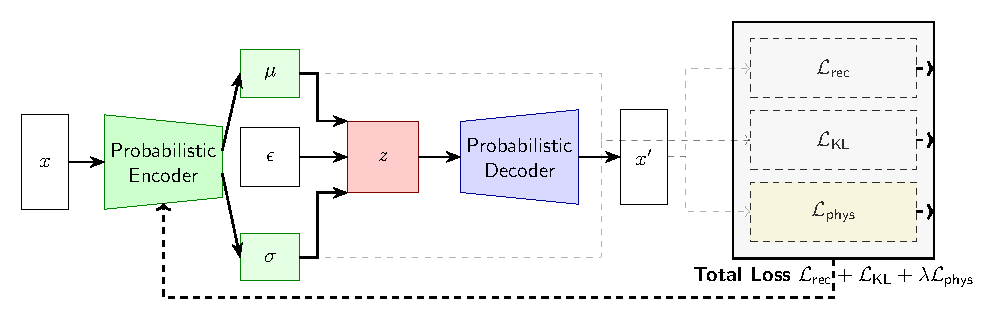
\includegraphics[width=0.95\linewidth]{fig/pinn_vae_go.pdf}
    \caption{Proposed PINN-VAE Diagram}
    \label{fig:diagram-losses}
\end{figure}

% Variational Inference (VI) in VAEs helps approximate the true underlying patterns of complex data by estimating how likely different data representations are, without directly solving computationally expensive problems.
% It enables VAEs to learn meaningful compressed represenations (latent variable) of data by balancing how well the data is recostructed and how simple is learned representation is.
% VI makes training VAEs efficient and scalable, allowing them to work with large datasets and uncover hidden structures without requiring exact solutions.

A \emph{probabilistic decoder} then maps the latent sample~$\mathbf z$ back to a reconstruction $\mathbf{x'}$ and simultaneously outputs the intermediate physiological variables
\(
\widehat T_{\text{core}},\;
\widehat T_{\text{skin}},\;
\widehat w
\)
as well as the target thermal-sensation vote $\widehat{\mathrm{TSV}}$. Admittedly, the combined dataset does not have $T_{skin}$ or $T_{core}$ let alone $\omega$ measured. Yet assisted by the \texttt{pythermalcomfort} package\cite{Tartarini_pythermalcomfort_2020}, %CITE THIS
we were able to calculate all three based on Gagge's two-node model\cite{gagge1986standard}, providing crucial connection back to the analytical relationship established in canonical research, completing the physiological piece that enables the current study to better regularize any potential issues with data quality, bias in data collection, etc.

\paragraph{Loss components}
The training objective combines three terms (illustrated at the right of Fig.~\ref{fig:diagram-losses}) with \gls{lrec} and \gls{lkl}:

    \begin{equation}
    L_{\text{rec}} = \lVert \mathbf x - \mathbf x' \rVert_2^{2}
    \end{equation}
    
    \begin{equation}    
    L_{\text{KL}}  = \tfrac12 \sum_{j}\!\bigl(\mu_j^{2} + \sigma_j^{2} - \ln\sigma_j^{2} - 1\bigr)\label{eq:kloss}
    \end{equation}
    
For the physiology-related penalty terms, let
\(
\operatorname{ReLU}(x)=\max(0,x)
\)
be the rectified–linear unit.  
For any predicted variable \(v\) with admissible range 
\([v_{\min},v_{\max}]\) 
we penalise only the out-of-bounds excess:

\begin{equation}
    \mathcal P(v;\,v_{\min},v_{\max})
        \;=\;
        \operatorname{ReLU}\!\bigl(v-v_{\max}\bigr)^{2}
        \;+\;
        \operatorname{ReLU}\!\bigl(v_{\min}-v\bigr)^{2}.
\end{equation}

\noindent
Squaring the ReLU output preserves differentiability everywhere
except at the range edges and gives a steeper gradient the farther the prediction drifts.

The full physiology loss, \gls{lphys} therefore becomes
\begin{equation}
  L_{\text{phys}} =
      \mathcal P\!\bigl(\widehat T_{\text{core}};\;36^{\circ}\text{C},\,38^{\circ}\text{C}\bigr)
    + \mathcal P\!\bigl(\widehat T_{\text{skin}};\;30^{\circ}\text{C},\,36^{\circ}\text{C}\bigr)
    + \mathcal P\!\bigl(\widehat w;\;0,\;0.7\ \text{kg\,h}^{-1}\bigr).\label{eq:phys_loss}
\end{equation}
\noindent
That is, we apply a \emph{ReLU‐squared} penalty whenever:
\begin{itemize}
    \item predicted core temperature falls below \(36^{\circ}\text{C}\) or exceeds \(38^{\circ}\text{C}\);
    \item predicted mean skin temperature leaves the \(30\mbox{–}36^{\circ}\text{C}\) known skin temperature band for indoor environment\cite{Fanger1970}; or
    \item predicted skin wettedness lies outside \(0\mbox{–}1.0\ \text{kg\,h}^{-1}\).
\end{itemize}


Because the ReLU term is zero inside the physiological range, the network is free to adjust intermediate variables so long as they remain biophysically plausible; once they breach the limits, the quadratic growth rapidly forces them back, making the constraint \emph{soft yet strongly binding}.  This is exactly the behaviour our earlier textual description (“ReLU this, not simple squared error”) was aiming for.


\paragraph{Total objective}
All terms are summed with equal physiology weights $\lambda_{\text{phys}}=0.33$:

\begin{equation}
    L_{\text{total}} = L_{\text{rec}} \;+\; L_{\text{KL}} \;+\; \lambda_{\text{phys}}\,L_{\text{phys}}.\label{eq:totloss}
\end{equation}

\noindent
In practice, the $\lambda_{\text{phys}}$ factor assigns one third of the total loss budget to keeping the predicted physiological signals within realistic limits, preventing the network from “hallucinating” impossible human states while it learns to impute missing person-specific data and to predict TSV accurately.

\paragraph{PPI overhead}
To make use of those records that still contain reliable person--specific information we prepend a \emph{personal–profile interface} (PPI). Each profile is a six--element vector
\(
  \mathbf p=
  \bigl[
     a,\;g,\;h,\;m,\;I_{cl},\;M_{\text{rest}}
  \bigr]
\)
(age, gender, height, weight, clothing factor and metabolic rate reported in the databases).  A learnable linear map
\(E:\mathbb R^{6}\!\rightarrow\!\mathbb R^{16}\) produces an
embedding
\(\tilde{\mathbf p}=E\mathbf p\),
which is concatenated with the main feature stream \(\mathbf x\). The encoder therefore minimises the same objective as Equation~\ref{eq:totloss}, but conditioned on the augmented input:
% \[
%   \boxed{%
%     \;L_{\text{total}}
%     = L_{\text{rec}}
%       + L_{\text{pred}}
%       + \lambda_{\text{reg}}\,L_{\text{KL}}
%       + \lambda_{\text{phys}}\,L_{\text{range}}
%   }\!,
%   \qquad
\begin{equation}
  q_{\phi}(\mathbf z)=q_{\phi}\bigl(\mathbf z\mid[\mathbf x,\tilde{\mathbf p}]\bigr).
\end{equation}
If a row lacks any personal variables the PPI block is bypassed (\(\tilde{\mathbf p}=\mathbf 0\)), so low–quality profiles can never degrade performance.


\subsection{Physiological Constraints and Basal Metabolic Rate Estimation}\label{sec:Physiological_Constraints}
Before setting out to assess the power of including more personal details, we first assessed the predictive power of updating the benefit of additional predictive power that can be harvested by more personal contextual factors if they're filled: the metabolic rate.  All of the metabolic rate levels reported in the combined dataset were activity indicator where 1.0 points to occupant in sedentary position. Yet as recent research are pointing to, there is an obvious need to address the underlying assumption of heat production hidden behind the 58.2$W/m^2$ assumption. 

We therefore went ahead and fed the untreated null-value-plagued data to a 10-fold lightgbm model first, and then compared it against three different variations of basal metabolic rate equations, by letting\(
m\,[\text{kg}]
\) be body mass,
\(
h\,[\text{cm}]
\) body height, and
\(
a\,[\text{yr}]
\) age.  
BMR is expressed in \emph{kcal\,day$^{-1}$}.  
Sex‐specific constants follow the original publications.

\paragraph{(1) Revised Harris–Benedict (Roza \& Shizgal, 1984\cite{Roza1984})}
\begin{align}
\mathrm{BMR}_{\mathrm{HB},\;\text{male}}   &= 88.362 \;+\; 13.397\,m \;+\; 4.799\,h \;-\; 5.677\,a, \\\label{eq:firstbmr}
\mathrm{BMR}_{\mathrm{HB},\;\text{female}} &= 447.593 \;+\; 9.247\,m \;+\; 3.098\,h \;-\; 4.330\,a.
\end{align}

\paragraph{(2) Mifflin–St Jeor (1990)\cite{Mifflin1990}}
\begin{align}
\mathrm{BMR}_{\mathrm{MSJ},\;\text{male}}   &= 10\,m \;+\; 6.25\,h \;-\; 5\,a \;+\; 5, \\
\mathrm{BMR}_{\mathrm{MSJ},\;\text{female}} &= 10\,m \;+\; 6.25\,h \;-\; 5\,a \;-\; 161.
\end{align}

\paragraph{(3) Livingston–Kohlstadt (2005) \textnormal{(adult subset, 19–50 yr)}\cite{Livingston2005}}
\begin{align}
\mathrm{BMR}_{\mathrm{LK},\;\text{male}}   &= 864 \;-\; 9.72\,a \;+\; 14.2\,m \;+\; 503\,\Bigl(\tfrac{h}{100}\Bigr),\\
\mathrm{BMR}_{\mathrm{LK},\;\text{female}} &= 387 \;-\; 7.31\,a \;+\; 10.9\,m \;+\; 660\,\Bigl(\tfrac{h}{100}\Bigr).
\end{align}
(The height term is expressed here with \(h\) in metres to match the original units.)


Body-surface area (BSA) is calculated with the classic Du Bois \& Du Bois (1916) relation
\begin{equation}
    \mathrm{BSA}\;[\text{m}^2] \;=\; 0.007184 \;
            m^{0.425}\;
            h^{0.725},
\end{equation}\label{eq:last-bmr}
again using \(m\) in kilograms and \(h\) in centimetres.

Resting metabolic power density is obtained by converting kilocalories per day to watts
\((1\ \text{kcal\,day}^{-1}=0.0484259\ \text{W})\) and dividing by BSA:
\begin{equation}
    M_{\mathrm{rest}}\;[\text{W\,m}^{-2}] \;=\;
    \frac{\mathrm{BMR}\;\times\;0.0484259}{\mathrm{BSA}}.
\end{equation}\label{eq:dubois}

Equation~\ref{eq:firstbmr} through~\ref{eq:last-bmr} allows us to calculate the corresponding basal metabolic rate, whereas Equation~\ref{eq:dubois} allows us to convert the basal metabolic rate to $W/m^2$\cite{DuBois1916}, which enables us to calculate three different sets of metabolic rates for the occupants: Multiplying the newly-obtained BMRs with the \texttt{metabolic\_rate}, since the latter is in fact the activity levels.

The PINN-VAE architecture also incorporates physiological constraints to guide the imputation and prediction process towards biophysically plausible states. These constraints are implemented via penalty terms in the loss function (detailed in Section~\ref{sec:PINN_VAE_Arch}, Eq.~\ref{eq:phys_loss}), applied to intermediate model outputs representing core temperature \gls{tcore} ($\hat{T}_{core}$), mean skin temperature \gls{tskin} ($\hat{T}_{skin}$), and skin wettedness \gls{wettedness} ($\hat{w}$).

The specific ranges used for these constraints, namely $T_{core} \in [36, 38]^{\circ}\text{C}$ and $T_{skin} \in [30, 36]^{\circ}\text{C}$, were chosen based on established principles of human thermoregulation and widely accepted values within the thermal comfort field. Human core temperature is tightly regulated around 37$^{\circ}$C, with the 36–38$^{\circ}$C range representing typical bounds under varying metabolic and environmental conditions while avoiding hypo- or hyperthermia. The mean skin temperature range of 30–36$^{\circ}$C encompasses values observed across different thermal states, from peripheral vasoconstriction in cooler environments (leading to lower $T_{skin}$) to vasodilation in warmer conditions (higher $T_{skin}$). Temperatures around 33–34$^{\circ}$C are frequently associated with thermal neutrality in standard indoor environments. These ranges are consistent with values discussed in key thermal comfort standards and foundational literature \cite{ASHRAE55,Fanger1970,gagge1986standard}. The skin wettedness constraint ($w \in [0, 1.0]$ based on typical calculation, reflects physical limits on sweat generation and evaporation. %Did I say 0.7 anywhre? 

\subsection{Evaluation Metrics: Direction-Penalty Statistic}
Our proposed PINN-VAE models consistently outperform unconstrained methods near thermal neutrality—where prediction errors have the greatest impact on occupant experience—and offer bounded physiological outputs, reducing the risk of implausible inference. To probe this behaviour better we built a “goal-post” test centred on thermal neutrality (|TSV| $\leq$ 0.5), i.e the \gls{neutralzone}:
\begin{itemize}
    \item Neutral hit. We record the share of cases in which the model and the occupant are both neutral.
    \item Right-direction miss. If the occupant feels slightly warm ( TSV > 0.5 ) or cool ( TSV < –0.5 ) we check whether the model errs in the same warm–cool direction and measure the mean absolute distance to zero for those rows.
    \item {Wrong-direction miss.} Rows where the sign is flipped are counted separately and their error magnitude is also averaged.
\end{itemize}
This framework allows us to further examine this beyond the neutral/right/wrong direction misses into a "direction-penalty statistic system. Using the predictions stitched from out-of-sample test set within the 5-fold CV, we split each record into cases where the model’s warm–cool sign matched the occupant and cases where it was reversed, computed the MAE for each subset, and formed their difference following:

\[
\Delta_{\text{dir}}
     = \text{MAE}_{\text{wrong sign}}
       \;-\;
       \text{MAE}_{\text{right sign}} .
\]

Following this framework, positive values mean the model’s error balloons when it crosses to the wrong side of neutral; values near zero (or negative) indicate that a sign flip does not add extra penalty.  To judge sampling uncertainty we drew 1,000 bootstrap resamples of the same rows and re-computed the difference each time, giving a non-parametric 95\% confidence band.

\subsection{Model Training and Evaluation Protocol Used}

We first proceeded our investigation with the non-filled dataset and trained a LightGBM regressor in a stratified 10-fold \gls{cv}. For each fold, BMR features (Harris-Benedict, Mifflin–St Jeor, Livingston-Kohlstadt) were added to the training split, the model was fit, and predictions on the held-out fold were stored. After all folds, the out-of-sample predictions were concatenated to form a single inference set. Comparing this set against the baseline (identical pipeline without any BMR values) isolates the marginal effect of metabolic-rate features via pure ablation. For model input, continuous features were standardized, and categorical features (e.g., \texttt{building\_type}, \texttt{season}) were converted into numerical representations using one-hot encoding, resulting in approximately 380 input features for the models.

Moving onwards to our PINN model. As illustrated in Figure~\ref{fig:diagram-losses}, the network keeps to a simple, fully-connected pattern. After one-hot encoding we feed roughly 380 numeric inputs, and—when person-specific information is available—append a 16-dimension embedding of age, gender, height, weight, clothing and metabolic rate.  The encoder reduces this combined vector to 128 units, then 64, each step using ReLU and a 0.1 dropout.  Two parallel heads map the 64 units to the latent mean $\mu$ and log-variance log $\sigma^2$.  A single latent size controls capacity; we searched {4, 8, 16} and found eight dimensions to give the lowest validation loss without over-fitting.  The decoder mirrors the encoder (64 $\rightarrow$ 128) and finally projects back to the original feature count plus four targets—the thermal-sensation vote and the three physiological intermediates.  All hidden layers share weights when the PPI block is disabled, so the only difference between the “plain” and “PPI” variant is whether that 16-D embedding is concatenated. These specific hyperparameter values (latent dimension $z=8$, $\lambda_{KL}=0.1$, $\lambda_{phys}=0.33$) were selected as they provided a stable balance between reconstruction fidelity, regularization, and predictive performance on validation sets during preliminary tuning phases. The core findings regarding neutral-zone performance and physiological plausibility appeared reasonably robust to minor variations around these selected values.

Training uses Adam ($1\times10^{-4}$), 50 epochs, batch size 64 and L2 gradient clipping at 1.  The loss combines reconstruction and prediction errors, a KL regulariser (weighted 0.1) and the physiology penalty, whose three components—core temperature, skin temperature and skin-wettedness—share equal weight so that each contributes the same influence.

Performance of PINN-family models are reported through a five-fold cross-validation.  For every fold we fit the scaler, the bounds and the network on 80 \% of the data, monitor loss on the held-out 20 \%, and keep the weights from the best epoch.  After all five folds we stitch the out-of-sample predictions back together, giving a single inference set for headline RMSE and MAE, and we retain the best fold’s weights to impute the full dataset that is released with the paper.

Regarding the models that we will be comparing, beyond the simple baseline \gls{pce} as reported by the combined dataset as they were from ASHRAE II and Chinese DB, we will be comparing three engines of models:

    \begin{itemize}
        \item \textit{lightgbm}: the base lightgbm model with no treatment on missing data,
        \item \textit{pv-pen}: our proposed architecture the \textbf{PINN--VAE},
        \item \textit{pvp-pen}: the \textbf{PINN--VAE--PPI} described above, and 
        \item \textit{ultra} lightgbm model trained on the fully imputed feature set from pv-pen/pvp-pen (whichever performs better in term so RMSE \& MAE.
    \end{itemize}

Metrics are reported (a) in one-vote TSV bins (\(-3\le\mathrm{TSV}\le+3\) with width 1) to expose
comfort-zone behaviour, and (b) in data-completeness bands (\(<30\%\), \(30\!-\!70\%\), \(>70\%\) of person fields present), with an additional split by which of the six PPI variables are available.  The classical PMV\(_{\text{CE}}\) equation is kept as a legacy baseline; when its error proved an order of magnitude larger in pilot runs we omitted it from detailed plots to preserve visual clarity while still stating its headline statistics in the text.
